\section{提出的方法}\label{ux63d0ux51faux7684ux65b9ux6cd5}

在多标签眼科疾病识别的域泛化过程中，模型性能主要受到三方面因素影响。首先，同一眼底图像中可能同时存在多种疾病，若模型不能有效建模疾病标签之间以及标签与疾病特征之间的关联，容易产生误检与漏检，从而降低多标签识别性能。其次，源域与目标域之间通常存在分布差异，若模型学习到的特征中包含较多源域特定噪声，则会削弱疾病相关特征的迁移能力，导致域泛化性能下降。此外，医疗数据隐私敏感，训练过程中产生的梯度或参数可能带来隐私泄露风险，需要在训练流程中引入隐私保护机制；但隐私保护机制通常会通过额外的训练约束影响模型优化过程，因此需要考虑隐私保护与模型性能之间的平衡问题。

针对上述问题，本文不将多疾病共存和域偏移视为两个孤立问题，而是统一到多标签眼科疾病识别的单域泛化框架中进行建模。如\figref{fig:method-framework}所示，所提可解释单域泛化框架主要包括两个部分：Part1.双分支引导域不变特征提取，Part2.自适应标签-特征关联性构建。Part1 以 CAM 作为引导，结合双分支 mask 对比学习机制，从单一源域中提取更稳定的域不变特征，缓解源域与未知域之间的分布差异影响。同时 CAM 能够可视化模型关注区域，增强可解释性；Part2 在 Part1 输出的域不变特征基础上，利用 Transformer 注意力机制建模标签-标签关联与标签-特征关联性，减少多标签识别中的误检与漏检。两个部分并非独立工作，而是通过特征过滤和注意力一致性约束形成协同：Part1 为 Part2 提供更稳定的域不变特征，Part2 进一步约束双分支注意力特征的一致性，从而共同提升域泛化性能。最后，训练过程中集成自适应高斯差分隐私机制，以缓解隐私保护机制对模型性能的影响，并在隐私保护与模型性能之间取得平衡。综合以上，所提方法构建了一个面向多标签眼科疾病识别的可解释与隐私保护单域泛化框架。以下分三小节详细描述各模块的实现细节。

\begin{figure}[!htb]
\centering
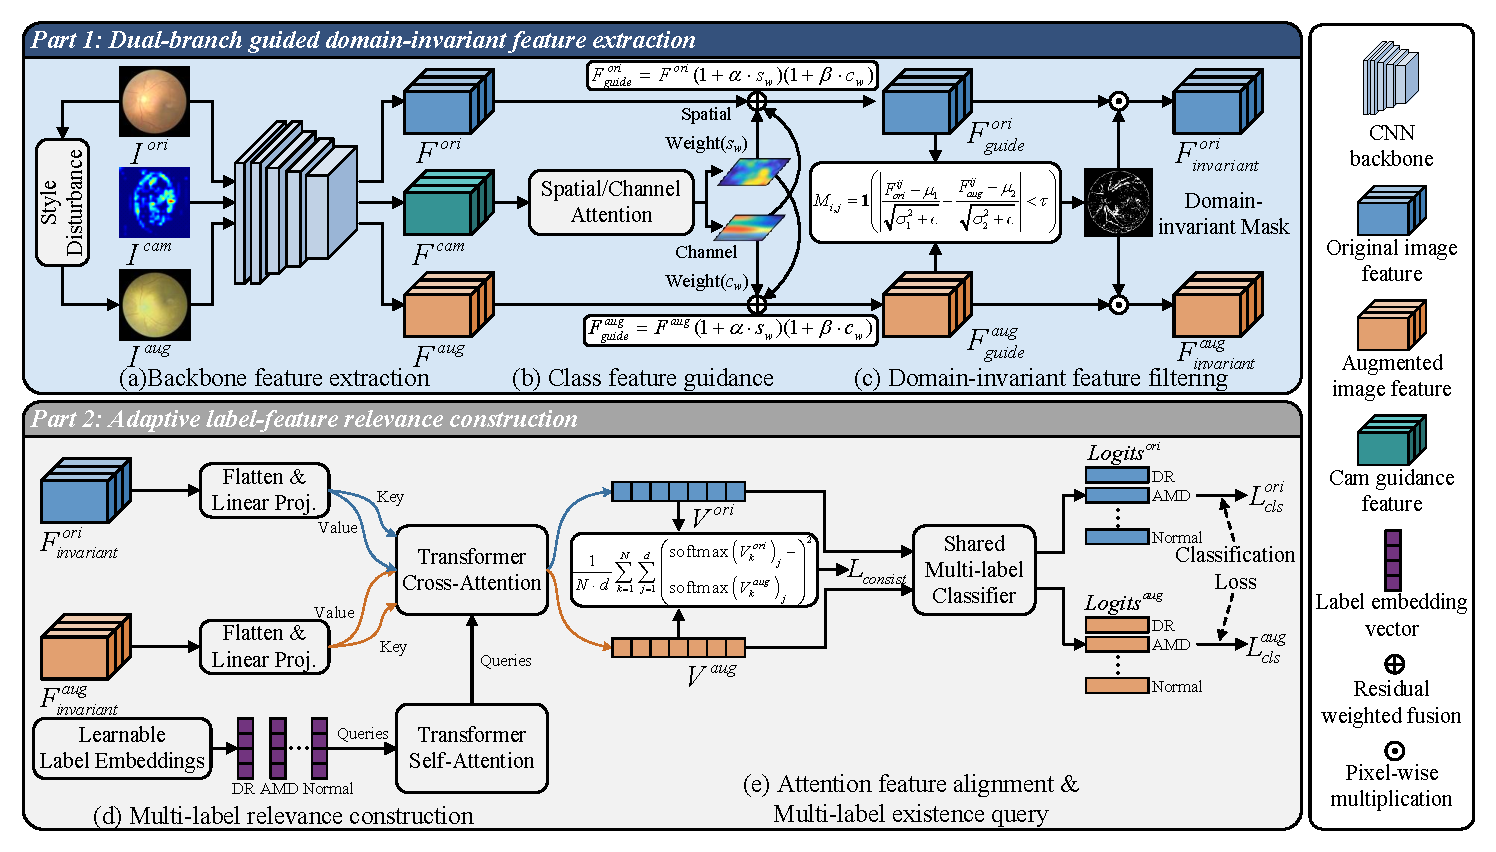
\includegraphics[width=0.96\textwidth]{./images/media/image2_padded.pdf}
\caption{所提可解释单域泛化框架总览。Part1 为双分支引导域不变特征提取（DFE），由 (a)--(c) 组成：首先 (a) 将源域原始图像与源域增强图像输入骨干网络提取双分支特征；同时 (b) 利用 CAM 生成模型关注区域引导，以增强疾病相关区域并抑制背景噪声；最终 (c) 通过双分支 mask 对比学习机制保留两路特征中的高度相似部分，从而提取域不变特征。Part2 为自适应标签-特征关联性构建（ARC），由 (d)--(e) 组成：其中 (d) 利用 Transformer 自注意力机制建模标签-标签关联，再通过交叉注意力机制建立标签-特征关联性，然后由 (e) 利用注意力一致性约束提升注意力特征的稳定性，从而减少多标签识别中的误检与漏检。Part1 和 Part2 协同工作，模型能够在提取域不变特征的同时更有效地建模标签关联，从而共同提升域泛化性能。}
\label{fig:method-framework}
\end{figure}

\letteredsubsection{A. 双分支引导域不变特征提取}

考虑到医疗场景中多机构数据往往难以集中或同步使用，本文采用单域泛化设置，仅利用一个源域学习面向未知域数据的域不变特征。受对比学习启发，本文将源域原始图像通过风格扰动等增强技术生成源域增强图像，用于模拟未知域可能出现的分布差异。具体而言，\(I^{ori}\)代表源域原始图像，而\(I^{aug}\)代表源域增强图像，通过风格扰动（如 MixStyle 方法或随机调整亮度、对比度、饱和度）生成。这种增强模拟了跨域场景中的成像设备、光照环境或患者群体差异，但保留了图像的语义内容（疾病区域）。

首先，如\figsubref{fig:method-framework}{a}部分所示，\(I^{ori}\)和\(I^{aug}\)二者共同送入骨干网络提取特征得到\(F^{ori}\)和\(F^{aug}\)。令\(F^{ori} \in \mathbb{R}^{C \times H \times W}\)和\(F^{aug} \in \mathbb{R}^{C \times H \times W}\)，其中\(C\)、\(H\)、\(W\)分别为骨干网络最终特征图的通道数、高度和宽度。本方法选择 ResNet50 \hyperref[_RefResNet2016]{{[}44{]}}作为骨干网络，因为其在图像识别任务中表现出色，具有较好的特征提取能力和计算效率。然而，仅依靠源域原始图像与源域增强图像之间的对比约束作用仍然有限，模型可能同时学习到背景纹理、光照变化或边缘伪影等域特定噪声，进而影响未知域上的多标签眼科疾病识别。

为此，我们引入\figsubref{fig:method-framework}{b}部分的类别特征引导模块，以提升特征的疾病相关性和可解释性。预先使用基线模型（ResNet50 + BCE 损失）在训练集上生成 CAM。CAM 突出模型对不同疾病区域的关注，例如糖尿病视网膜病变（DR）关注血管区，年龄相关性黄斑变性（AMD）关注黄斑区。其计算公式为：

\begin{equation}\label{eq:cam}
I^{cam} = \sum_{k = 1}^{C}w_{k} \cdot A_{k},
\end{equation}
其中\(A_{k}\)是骨干网络最后一层卷积的第\(k\)个通道激活图，\(w_{k}\)是通过全局平均池化后对分类权重的梯度计算得到的权重。该公式基于 Grad-CAM 变体，确保 CAM 捕捉类别特定模型关注区域。生成的 \(I^{cam}\)输入骨干网络得到\(F^{cam} \in \mathbb{R}^{C \times H \times W}\)，然后通过空间/通道注意力模块分别计算\(F^{cam}\)的空间注意力权重\(s_{w}\)和通道注意力权重\(c_{w}\)。两个注意力模块均为卷积序列网络，均包含1x1 卷积、ReLU 激活和 Sigmoid 函数，用于自适应生成权重。空间注意力模块额外结合平均/最大池化捕捉局部上下文，从而生成像素级权重图，自适应放大病变区域（如血管或黄斑）的显著性，同时抑制背景噪声。通道注意力模块则采用自适应平均池化压缩空间维度以获取全局统计，随后学习通道依赖，从而增强疾病纹理敏感通道的权重，抑制噪声通道。分别将两权重加权应用到\(F^{ori}\)和\(F^{aug}\)得到 CAM 引导特征\(F_{guide}^{ori}\)和\(F_{guide}^{aug}\)，具体的加权方式采用残差连接机制，避免过度引导破坏原始信息。公式为：

\begin{align}
F_{guide}^{ori} &= F^{ori}(1 + \alpha{\cdot s}_{w})(1 + {\beta \cdot c}_{w}), \label{eq:guide-feature-ori} \\
F_{guide}^{aug} &= F^{aug}(1 + \alpha{\cdot s}_{w})(1 + {\beta \cdot c}_{w}), \label{eq:guide-feature-aug}
\end{align}
其中\(\alpha\)和\(\beta\)分别为控制\(s_{w}\)和\(c_{w}\)增强程度的超参数。残差加权方式使 CAM 引导信息在保留原始特征表达的同时突出疾病相关区域，减少模型对光照、背景纹理等域特定噪声的依赖。在此基础上再提取域不变特征，有助于提升特征的疾病相关性；同时 CAM 的模型关注区域可视化也增强了模型的可解释性，帮助临床医生理解预测依据，例如通过叠加 CAM 观察模型是否关注病变区域。

接下来是域不变特征过滤模块，如\figsubref{fig:method-framework}{c}所示。本文采用双分支 mask 对比学习机制，将源域原始图像引导特征和源域增强图像引导特征在特征分布层面计算相似度，相似度高的部分代表在风格扰动下仍保持稳定的疾病相关区域，予以保留；相似度低的部分更可能包含光照、设备风格或风格扰动带来的域特定噪声，予以抑制。掩码矩阵\(M \in \mathbb{R}^{C \times H \times W}\)的计算基于标准化距离：

\begin{equation}\label{eq:mask}
M_{ij} =
\left\{
\begin{array}{ll}
1, & \text{if } \left| \dfrac{F_{guide}^{ori,ij} - \mu_{1}}{\sqrt{\sigma_{1}^{2} + \epsilon}} - \dfrac{F_{guide}^{aug,ij} - \mu_{2}}{\sqrt{\sigma_{2}^{2} + \epsilon}} \right| \leq \tau, \\
0, & \text{otherwise.}
\end{array}
\right.
\end{equation}
其中\(\mu_{1},\sigma_{1}\)和\(\mu_{2},\sigma_{2}\)分别是两个引导特征的均值和方差，\(\epsilon = 10^{-5}\)为稳定性常数，\(i,j\)表示特征图位置。然后根据阈值\(\tau\)将相似部分置1，不相似置0。最终将掩码矩阵分别应用到\(F_{guide}^{ori}\)和\(F_{guide}^{aug}\)提取域不变特征，具体为：

\begin{equation}\label{eq:invariant-feature}
F_{invariant}^{ori} = F_{guide}^{ori} \odot M,F_{invariant}^{aug} = F_{guide}^{aug} \odot M,
\end{equation}
其中\(\odot\)是像素级逐元素乘法，确保只保留共有的疾病相关特征，如血管或黄斑区纹理，而剔除光照或设备噪声。由此得到的\(F_{invariant}^{ori}\)和\(F_{invariant}^{aug}\)作为后续标签-特征关联性构建的输入，使多标签关联学习建立在更稳定的域不变特征之上。

\letteredsubsection{B. 自适应标签-特征关联性构建}

在获得域不变疾病特征后，模型将进一步处理眼科疾病共存带来的多标签关联问题。为此，本文嵌入 Transformer 注意力机制，在标签和特征层面构建自适应关联，实现多标签预测。具体模块如\figsubref{fig:method-framework}{d}和\figsubref{fig:method-framework}{e}所示，包括多标签关联构建和注意力特征对齐。

首先，将8类标签（ODIR 数据集：正常、DR、AMD 等）建模为可学习向量\(L = \lbrack L_{1},\ldots,L_{8}\rbrack \in \mathbb{R}^{8 \times d}\)，其中\(d = 512\)是嵌入维度。这些向量初始化为随机高斯分布，并在训练中优化，便于刻画不同疾病标签之间的潜在关联。标签向量输入到 Transformer 自注意力机制（Self-Attention），建模标签关联：

\begin{equation}\label{eq:self-attention}
V_{self} = \operatorname{softmax}\left(\frac{QK^{T}}{\sqrt{d_{k}}}\right)V,
\end{equation}
其中\(Q = LW_{Q},K = LW_{K},V = LW_{V}\)，\(W_{Q},W_{K},W_{V}\)是可学习投影矩阵，\(d_{k} = d/heads\)（多头注意力，heads=8）。自注意力输出\(V_{self}\)用于捕捉标签关联，使不同疾病标签能够根据训练数据中的共现模式和视觉证据进行动态交互。

接下来，使用交叉注意力机制（Cross-Attention）将标签与域不变特征结合。因为 Transformer 需要接收序列输入，我们先将 Part1 输出的\(F_{invariant}^{ori}\)和\(F_{invariant}^{aug}\)展平（Flatten），作为 Key 和 Value，与标签向量\(V_{self}\)作为 Query，进行交叉注意力计算。计算公式为：

\begin{equation}\label{eq:cross-attention}
V_{cross}^{ori} = \operatorname{softmax}\left(\frac{V_{self}W_{Q}(F_{invariant}^{ori}W_{K})^{T}}{\sqrt{d_{k}}}\right)(F_{invariant}^{ori}W_{V}),
\end{equation}
类似计算\(V_{cross}^{aug}\)。通过交叉注意力加权，标签与对应疾病特征进行匹配，形成注意力向量\(V \in \mathbb{R}^{8 \times d}\)，使每个标签向量在疾病相关区域上获得更高响应。在这一过程中，每个标签向量并不是独立地与图像特征进行匹配，而是在自注意力机制建模后的标签关联基础上进行查询。因此，模型既能关注单个疾病对应的局部病灶特征，也能利用疾病共现依赖辅助判断其他相关标签，从而减少多标签识别中的误检与漏检。

为了确保双分支向量输出一致，我们引入注意力一致性约束，并计算注意力一致性损失。源域原始图像和源域增强图像具有相同的疾病标签，只是二者存在风格差异，因此对应的标签注意力向量也应保持接近。该损失通过约束两条分支的注意力特征一致，使模型在不同风格输入下仍学习到相近的标签-特征关联性。具体计算方式为均方误差（MSE），公式为：

\begin{equation}\label{eq:consistency-loss}
L_{consist} = \frac{1}{N \cdot d}\sum_{k = 1}^{N}\sum_{j = 1}^{d}
\left(
\operatorname{softmax}\left( V_{k}^{ori} \right)_{j}
-
\operatorname{softmax}\left( V_{k}^{aug} \right)_{j}
\right)^{2},
\end{equation}
其中\(N = 8\)是标签数，\(d = 512\)是嵌入维度，Softmax 用于将注意力向量归一化为可比较的分布形式。注意力一致性损失通过最小化两分支归一化注意力特征之间的差异，提升模型在域偏移下的稳定性。

最终，注意力向量输入多标签分类器，首先对类别查询特征施加 LayerNorm 与 Dropout 进行轻量级特征增强，用于规范化和正则化查询特征，随后通过逐类别的线性变换获得每个类别的 logits，经 Sigmoid 激活后，得到各类别的预测概率\(p^{ori}\)，类似得到\(p^{aug}\)。分类损失采用二元交叉熵（BCE）：

\begin{equation}\label{eq:cls-loss}
L_{cls}^{ori} = - \frac{1}{8}\sum_{k = 1}^{8}{\lbrack y_{k}\log p_{k}^{ori} + (1 - y_{k})\log(1 - p_{k}^{ori})\rbrack},
\end{equation}
总损失为\(L = L_{cls}^{ori} + L_{cls}^{aug} + \lambda L_{consist}\)，其中\(\lambda\)为平衡一致性程度的超参数。通过上述设计，DFE 模块为 ARC 模块提供与疾病相关的域不变特征，ARC 模块进一步建模标签-标签关联性及标签-特征关联性，二者协同提升跨域场景下的多标签识别能力。

\letteredsubsection{C. 隐私保护集成}

医疗图像数据高度敏感，训练过程中产生的梯度或模型参数可能泄露样本信息，其中梯度逆向攻击甚至可能恢复原始图像，导致隐私泄露风险。考虑到单域泛化模型的隐私保护与模型性能的平衡问题，本文引入自适应高斯差分隐私（Adaptive Gaussian differential privacy, AdaGDP）机制。整体的隐私保护框架如\figref{fig:privacy-framework}所示。

\begin{figure}[!htb]
\centering
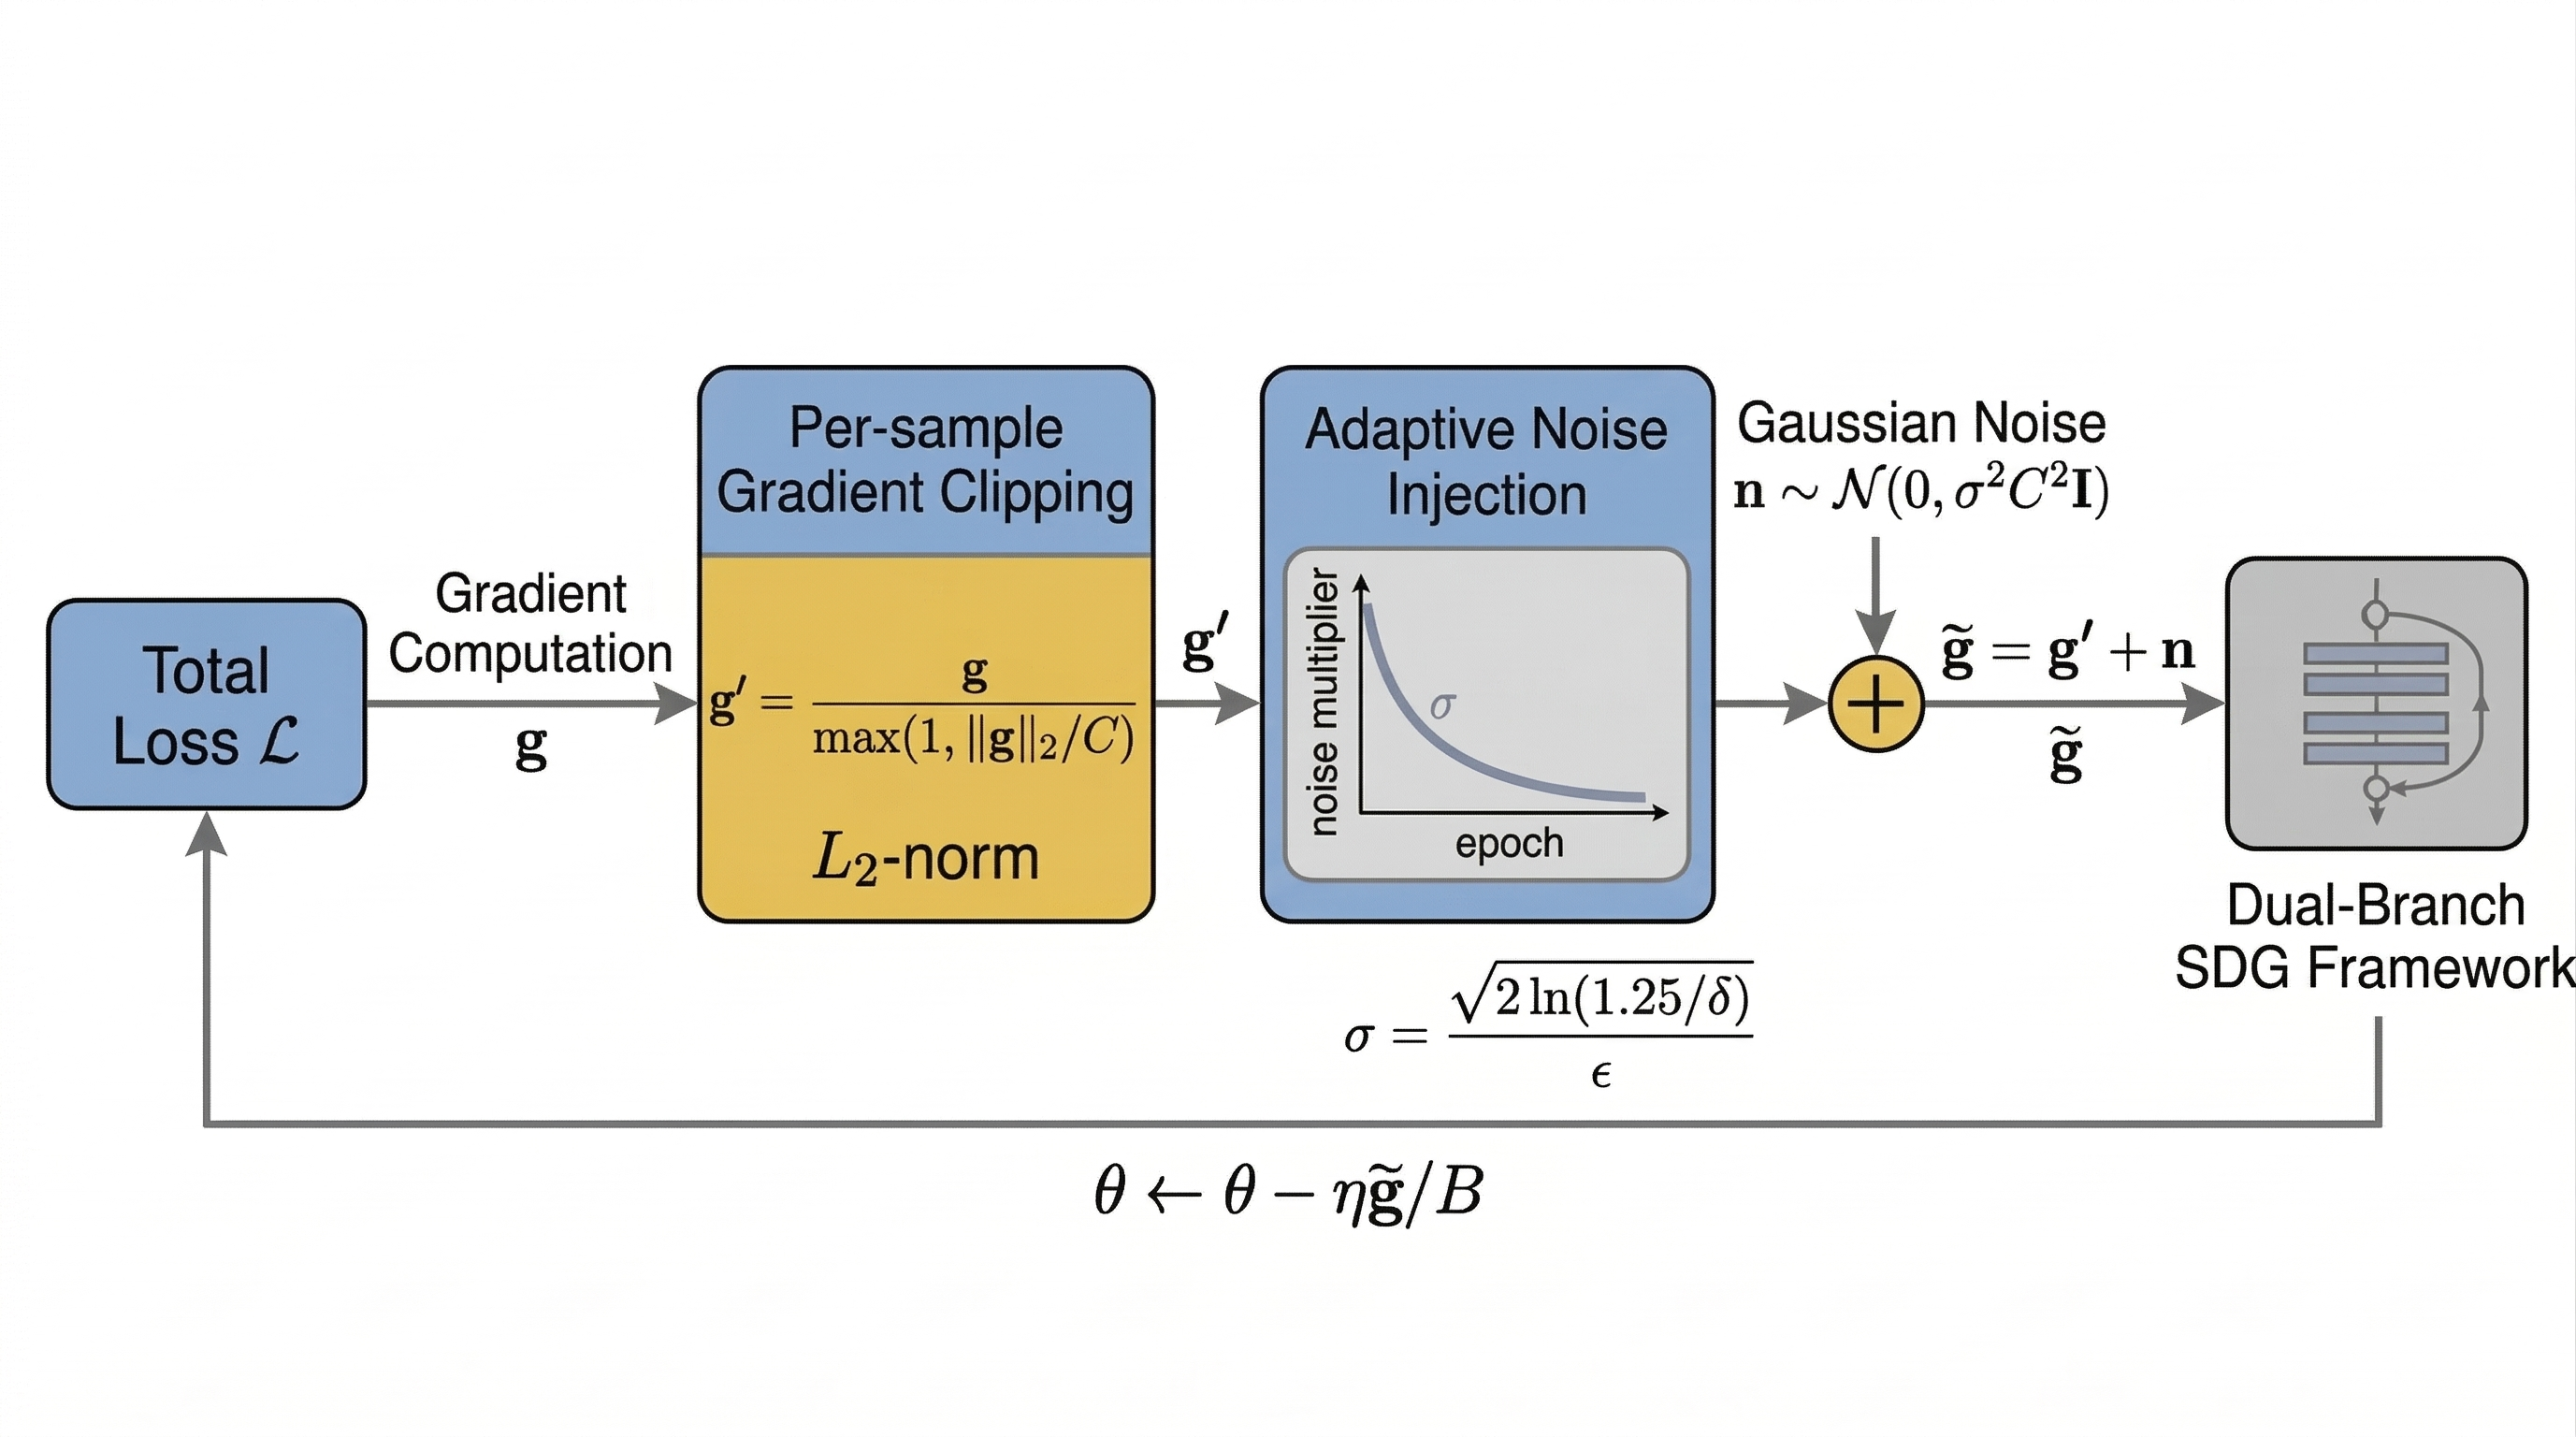
\includegraphics[width=0.82\textwidth]{./images/media/image3_v2.png}
\caption{自适应高斯差分隐私在单域泛化框架中的集成方式。训练过程中，每步更新均先对样本梯度进行裁剪，再注入高斯噪声并完成参数更新；与固定噪声差分隐私不同，本文采用随训练阶段自适应调整并逐步衰减的噪声乘数，从而在训练前期提供较强隐私保护，在训练后期减小噪声对模型收敛的干扰，进而取得隐私-性能平衡。}
\label{fig:privacy-framework}
\end{figure}

高斯差分隐私（Gaussian Differential Privacy, GDP）通过在每步梯度更新时加入独立同分布的高斯噪声实现\((\epsilon, \delta)\)-差分隐私。对于相邻数据集\(D\)和\(D'\)（仅相差一个样本），若随机算法\(M\)对任意输出集合\(S\)满足：

\begin{equation}\label{eq:dp-definition}
\Pr\lbrack M(D) \in S\rbrack \leq e^{\epsilon}\Pr\lbrack M(D') \in S\rbrack + \delta,
\end{equation}
则称\(M\)满足\((\epsilon, \delta)\)-DP，其中\(\epsilon\)衡量隐私保护程度，\(\delta\)为松弛项，通常设为\(10^{-5}\)。在 DP-SGD 框架下，每次迭代对每个样本梯度\(g\)先进行 L2 范数裁剪：

\begin{equation}\label{eq:gradient-clip}
g' = g/max(1, \parallel g \parallel_{2}/C),
\end{equation}
然后加入高斯噪声\(n \sim \mathcal{N}(0,\sigma^{2}C^{2}I)\)，其中\(\sigma\)为噪声乘数，用于控制噪声强度，通常与隐私预算\(\epsilon\)和松弛项\(\delta\)相关，可写为：

\begin{equation}\label{eq:noise-multiplier}
\sigma = \sqrt{2\ln(1.25/\delta)}/\epsilon.
\end{equation}
噪声梯度\(\widetilde{g} = g' + n\)，更新\(\theta \leftarrow \theta - \eta\widetilde{g}/B\)，其中\(B\)是批次大小。该过程通过注入噪声模糊梯度，防止逆向攻击恢复原始图像或标签。有关隐私保护机制及其安全性的详细证明，请参阅 Dwork C et al. \hyperref[_Ref214903493]{{[}45{]}}的工作。

然而，传统 GDP 在整个训练过程中使用固定\(\sigma\)，导致训练后期仍注入大量噪声，容易影响模型收敛和最终性能。为此，我们采用自适应高斯差分隐私优化器，在训练初期使用较大噪声乘数以提供较强保护，随后根据预设噪声衰减速率逐步降低噪声强度，以减小后期对模型收敛的影响。训练过程中，本文根据每轮噪声乘数、噪声衰减速率和采样过程累计隐私预算，并记录不同训练轮次下的\(\epsilon\)消耗与模型性能变化，用于分析隐私预算增长过程中的性能演化。最终实验验证，在中等隐私预算下，所提方法能够缓解噪声注入带来的性能下降，在隐私保护与模型性能之间取得较好的平衡。
